% TeX encoding = utf8
% TeX spellcheck = pl_PL 
\documentclass[a4paper, 11pt]{article}
\usepackage[utf8]{inputenc}
\usepackage[polish]{babel}
\usepackage{polski}
\usepackage{graphicx}
\usepackage{listings}
\usepackage{amsfonts}
\usepackage{geometry}
\usepackage{multicol}
\usepackage{latexsym}
\usepackage{enumerate}
\usepackage{hyperref}
\usepackage{color} %red, green, blue, yellow, cyan, magenta, black, white
\definecolor{mygreen}{RGB}{28,172,0} % color values Red, Green, Blue
\definecolor{mylilas}{RGB}{170,55,241}

\author{Kamil Foryszewski}
\title{Dokumentacja projektu laboratoryjnego numer 1 przedmiot MNUM}
\frenchspacing

\newgeometry{tmargin=2cm, bmargin=2cm, lmargin=2cm, rmargin=2cm}
\pagestyle{empty}


\begin{document}

\lstset{language=Matlab,%
    basicstyle=\color{red},
    breaklines=true,%
    morekeywords={matlab2tikz},
    keywordstyle=\color{blue},%
    morekeywords=[2]{1}, keywordstyle=[2]{\color{black}},
    identifierstyle=\color{black},%
    stringstyle=\color{mylilas},%
    commentstyle=\color{mygreen},%
    showstringspaces=false,
    numbers=right,%
    numberstyle={ \color{black}},% size of the numbers
    numbersep=5pt, % this defines how far the numbers are from the text
    emph=[1]{for,endfor,endwhile,endfunction,endif,break},emphstyle=[1]\color{blue}, %some words to emphasise
    emph=[2]{,.}, emphstyle=[2]\color{yellow},%
}

\maketitle
\tableofcontents


\section{Zadanie 1}

\subsection{Polecenie}

\vspace{0,5cm}

\subsection{Opis teoretyczny}
\indent

\begin{enumerate}
  \item $a = 1, b = 2$
  \item dopóki $a$ różne od $1$ $eps = x/2, b = 1 + x$
  \item wyświetl eps
\end{enumerate} 



\subsection{Realizacja w programie Matlab}



\vspace{1cm}

\subsection{Wynik działania programu}


	
\subsection{Wnioski}
\indent 



\section{Metoda elminacji Gaussa z częściowym wyborem elementu głównego}

\subsection{Polecenie}


\subsection{Opis teoretyczny}



$$
\left( \begin{array}{ccc}
a_{11}^T & a_{12} \\
a_{21} & A_{22} \\
\end{array} \right)
=
\left( \begin{array}{ccc}
1 & 0^T \\
l_{21} & L_{22} \\
\end{array} \right)
\left( \begin{array}{ccc}
u_{11} & u_{12}^T \\
0 & U	_{22} \\
\end{array} \right)
$$

Teraz mnożąc blokowo macierz $L$ przez $U$ :
\begin{itemize}
\item $u_{11} = a_{11}$ oraz $u_{12} = a_{12} \to $ pierwszy wiersz $U$ jest kopią pierwszego wiersza $A$
\item $l_{21} = a_{21}/u_{11} \to$ pierwsza kolumna $L$ powstaje przez podzielenie wektora $a_{2:}$ przez element na diagonali.
\item $A_{22} - l_{21}u_{12}^T = L_{22}U_{22} \to$ znalezienie podmacierzy $L_{22} , U_{22}$ sprowadza się do znalezienia rozkładu $LU$ zmodyfikowanego bloku $A_{22}$ macierzy $A$ o wymiarze $(n-1)\times(n-1)$. Procedurę tą nazywamy uzupełnieniem Schura.
\end{itemize}


\textbf{Złożoność obliczniowa}\\

\textbf{Realizacja w programie Matlab}\\
\\

\begin{lstlisting}

\end{lstlisting}


\subsection{Generowanie danych do obliczeń}


$$
1) \ a_{ij} = \left\{ \begin{array}{ll}
10 & \textrm{dla $i=j$,}\\
5 & \textrm{dla $i=j-1$ lub $i=j+1$, \hspace{1cm} $b_{i} = 2+0,3i$;}\\
0 & \textrm{dla pozostalych,}
\end{array} \right.
$$
\hspace{3cm} $2) \ a_{ij} = 2(i-j)+1$ \hspace{1cm} $a_{ii} = \frac{1}{6}$ \hspace{1cm} $b_{i} =1+0,4*i$; \\

\hspace{2,4cm} $2) \ a_{ij} = \frac{8}{9(i+j+1)}$  \hspace{1cm} $b_{i} =\frac{4}{3i}$ $i$ parzyste; $b_{i} = 0$ $i$ - nieparzyste; \\

\vspace{1cm}

\textbf{Realizacja w programie Matlab}\\
\\
\begin{lstlisting}

\end{lstlisting}

\subsection{Wyniki działania programu}


\textbf{Realizacja w programie Matlab}\\
\\
\begin{lstlisting}

\end{lstlisting}


\vspace{1cm}
\textbf{Zestaw danych 1}\\
\\


\vspace{2cm}
\textbf{Wnioski}\\

\textbf{Zestaw danych 2}\\
\\


\textbf{Wnioski}\\
\\
Dla drugiego zestawu danych błąd rozwiązania jest znacznie większy i rośnie wraz z liczbą równań. 
Elementy na diagonali są znacznie mniejsze co do modułu od pozostałych. Powoduje to pojawianie się wartości bliskich zeru podczas generowania macierzy $LU$, co prowadzi do dużych błędów w obliczeniach. Dla liczby równań powyżej 1280 czas potrzebny na rozwiąznie staje się zabyt długi. 




% \begin{figure}[th]
% 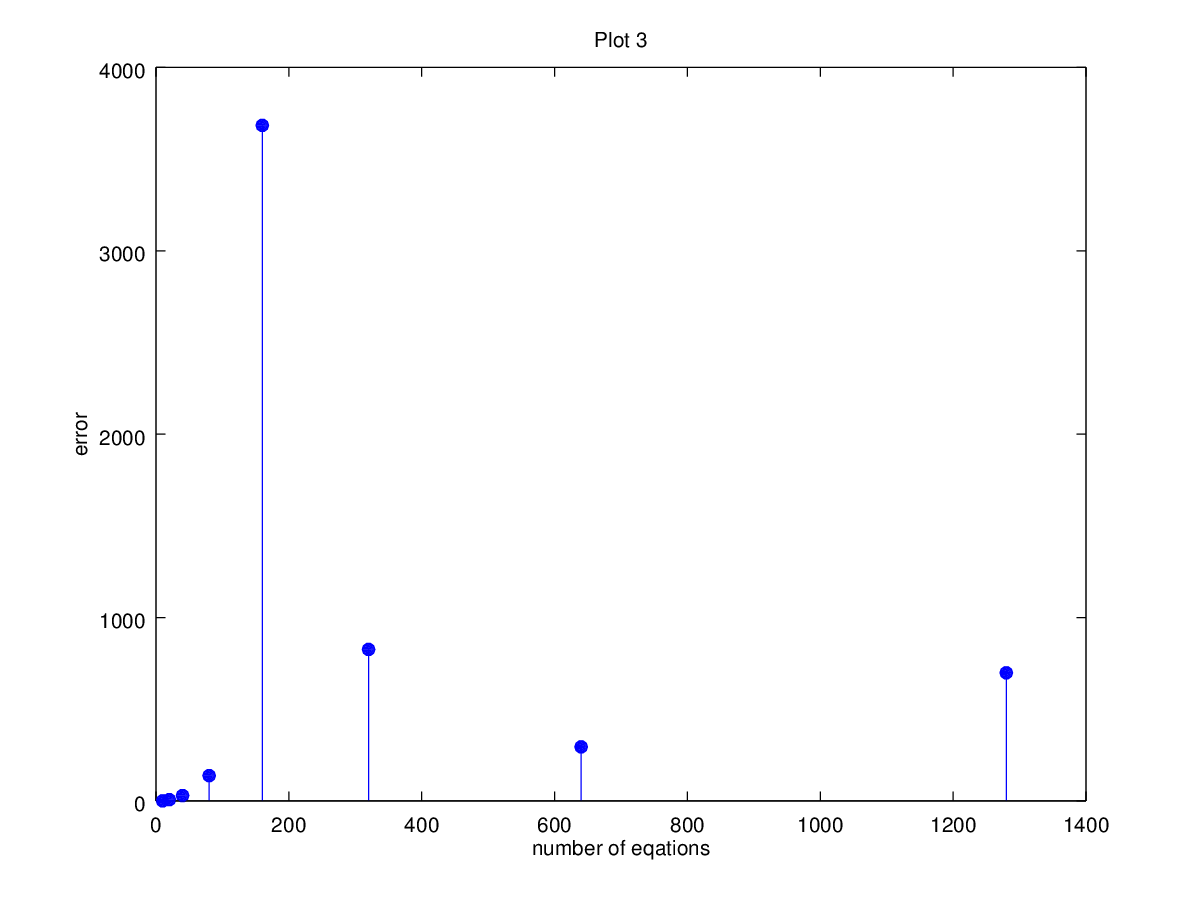
\includegraphics[width=\textwidth]{wykres3}
% \end{figure}

\vspace{1cm}
\textbf{Wnioski}\\




\begin{thebibliography}{99}
\bibitem{first} Piotr Tatjewski "Metody numeryczne": Rozdział 1.1\\
Warszawa 2013
\bibitem{second}
\url{https://en.wikipedia.org/wiki/Machine_epsilon}
\bibitem{third} Piotr Tatjewski "Metody numeryczne": Rozdział 2.3.4\\
Warszawa 2013
\bibitem{fourth} Piotr Tatjewski "Metody numeryczne": Rozdział 2.3.4 (2.29)\\
Warszawa 2013
\bibitem{fifth} Piotr Tatjewski "Metody numeryczne": Rozdział 2.3.5\\
Warszawa 2013
\bibitem{sixth} Piotr Tatjewski "Metody numeryczne": Rozdział 2.6.1\\
Warszawa 2013
\end{thebibliography}










	
\end{document}


